\section{Detalle Primera Iteración}

\subsection{Detalle y tareas de casos de uso}

A continuación se presenta una descripción de alto nivel de los casos de uso a 
desarrollar durante la primera iteración. Además, se define la lista de tareas 
relacionadas con cada CU.

\subsubsection{\underline{CU01: Enviando información del vehículo al servidor}}

Detalle: Se refiere a la acción de mandar los datos obtenidos por el gps de los 
vehículos al servidor de forma segura.


Tareas: 
\begin{itemize}

\item CU01-T01: Analizar volumen de datos

\item CU01-T02: Investigacion de tecnologias
\begin{itemize}
\item CU01-T02-st01: Seguridad
\item CU01-T02-st02: Concurrencia
\item CU01-T02-st03: Alto rendimiento
\end{itemize}

\item CU01-T03: Investigación de formas de comunicación
\begin{itemize}
\item CU01-T03-st01: Internet
\item CU01-T03-st02: Radiofrecuencia
\item CU01-T03-st03: GSM
\item CU01-T03-st04: Satelital (ArSAT)
\end{itemize}

\item CU01-T04: Configuración del ambiente de desarrollo (2 hs)
\item CU01-T05: Especificación de la información necesaria para generar las infracciones (4 hs)
\item CU01-T06: Implementación de mock del dispositivo del vehículo (2 hs)
\item CU01-T07: Configuración del ambiente de testing (2 hs)
\item CU01-T08: Testing (8 hs)

\end{itemize}

\begin{table}[htb]
\begin{center}
\begin{tabular}{|l|c|}
\hline
Tarea & Estimación (Horas Hombre) \\
\hline \hline
CU01-T01: Analizar volumen de datos & 2 \\ \hline
CU01-T02: Investigacion de tecnologias & 10 \\ \hline
CU01-T03: Investigación de formas de comunicación & 10 \\ \hline
CU01-T04: Configuración del ambiente de desarrollo & 2 hs \\ \hline
CU01-T05: Especificación de la información necesaria para generar las infracciones & 4 hs \\ \hline
CU01-T06: Implementación de mock del dispositivo del vehículo & 2 hs \\ \hline
CU01-T07: Configuración del ambiente de testing & 2 hs \\ \hline
CU01-T08: Testing & 8 hs \\ \hline
Total HH & 40 \\ \hline
\end{tabular}
\caption{Estimación de tiempo en horas hombre de las tareas del CU01}
\label{tabla:sencilla}
\end{center}
\end{table}


PONER GRAFO DE DEPENDENCIAS ENTRE TAREAS DEL CU01

\subsubsection{\underline{CU02: Detectando baja conectividad}}

Detalle: Se refiere a la acción de localizar las zonas en las cuales no hay buena 
conectividad, avisando al sistema ManejAR.


Tareas: 
\begin{itemize}

\item CU02-T01: Investigación de tecnologías para sensores
\begin{itemize}
\item CU02-T01-st01: Hardware
\item CU02-T01-st02: Software
\end{itemize}

\item CU02-T02: Implementar comunicación de los sensores con los servidores

\item CU02-T03: Implementar algoritmos de nivel de conectividad en el servidor 
\begin{itemize}
\item CU02-T03-st01: Definir qué se considera baja conectividad
\item CU02-T03-st02: Implementar algoritmo
\end{itemize}

\item CU02-T04: Implementación de mock del dispositivo de los sensores
\item CU02-T05: Implementar una demo para la empresa de Drones
\item CU02-T06: Configuración del ambiente de testing
\item CU02-T07: Testing

\end{itemize}

\begin{table}[htb]
\begin{center}
\begin{tabular}{|l|c|}
\hline
Tarea & Estimación (Horas Hombre) \\
\hline \hline
CU02-T01: Investigación de tecnologías para sensores & 6 \\ \hline
CU02-T02: Implementar comunicación de los sensores con los servidores & 8 \\ \hline
CU02-T03: Implementar algoritmos de nivel de conectividad en el servidor & 8 \\ \hline
CU02-T04: Implementación de mock del dispositivo de los sensores & 2 \\ \hline
CU02-T05: Implementar una demo para la empresa de Drones & 8 \\ \hline
CU02-T06: Configuración del ambiente de testing & 2 \\ \hline
CU02-T07: Testing & 6 \\ \hline
Total HH & 40 \\ \hline
\end{tabular}
\caption{Estimación de tiempo en horas hombre de las tareas del CU02}
\label{tabla:sencilla}
\end{center}
\end{table}

PONER GRAFO DE DEPENDENCIAS ENTRE TAREAS DEL CU02


\subsection{Tareas de la primera iteración}

Tareas primera iteración

Identificador de iteración: E01
Tipo de iteración: Elaboración
Tareas:

E01-T01: Diseño conceptual del sistema (4 hs)
E01-T02: Realización de WBS (8 hs)
E01-T03: Análisis de riesgos (3 hs)
E01-T04: Refinamiento de objetivos y requerimientos (16 hs)
E01-T05: Reconocimiento de casos de uso (3 hs)
E01-T06: Priorización de casos de uso (1 hs)
E01-T07: Estimación de tiempo de casos de uso (1 hs)
E01-T08: Análisis de atributos de calidad del sistema (6 hs)
E01-T09: Diseño de arquitectura del sistema (32 hs)
E01-T010: Elección de tecnologías (6 hs)
E01-T011: Realización de las tareas del caso de uso CU01 - Enviando información del vehículo al servidor (40 hs)
E01-T012: Realización de las tareas del caso de uso CU02 - Detectando baja conectividad (40 hs)

PONER EL CUADRITO DE LAS HH

\subsection{Gantt de la primera iteración}

A continuación se muestro el gráfico del gantt resultante bla bla bla.

%\centerline{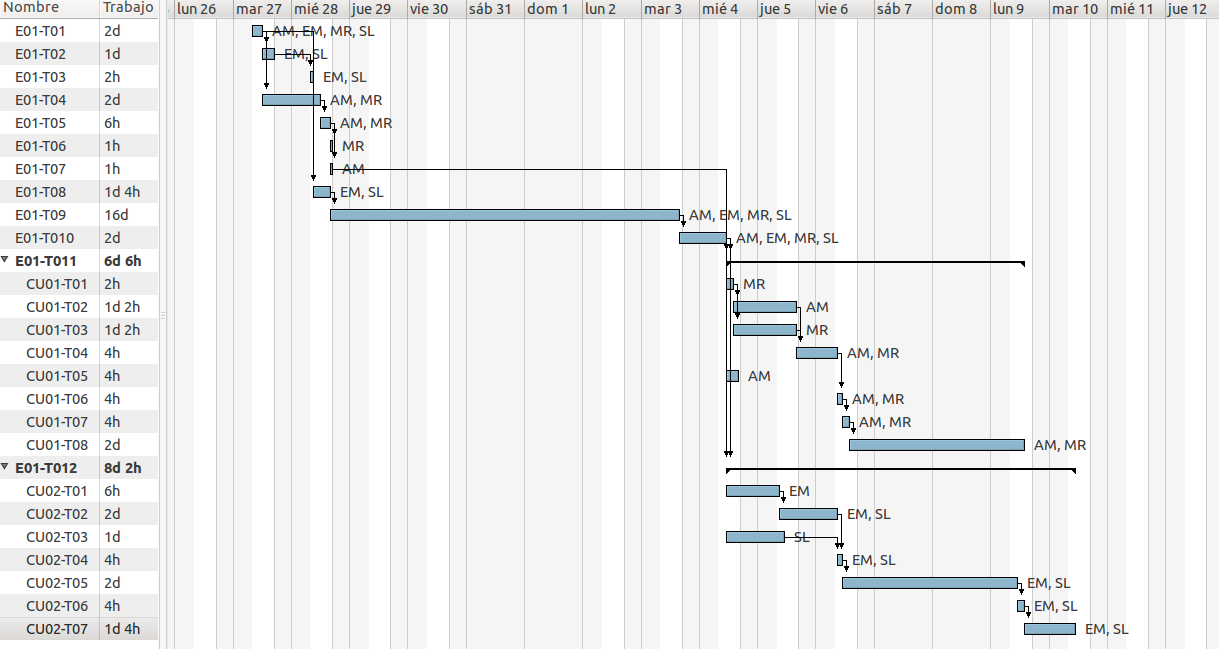
\includegraphics[width=1\textwidth]{./imagenes/gantt.png}}
